\documentclass[aspectratio=169]{beamer}

\usetheme{Madrid}
\usecolortheme{default}
\usepackage{graphicx}
\usepackage{listings}
\usepackage{xcolor}
\usepackage{booktabs}
\usepackage{tikz}
\usetikzlibrary{arrows.meta, positioning, calc}

% Custom colors
\definecolor{codegreen}{rgb}{0,0.6,0}
\definecolor{codegray}{rgb}{0.5,0.5,0.5}
\definecolor{codepurple}{rgb}{0.58,0,0.82}
\definecolor{backcolour}{rgb}{0.95,0.95,0.92}

% Code listing style
\lstdefinestyle{mystyle}{
    backgroundcolor=\color{backcolour},   
    commentstyle=\color{codegreen},
    keywordstyle=\color{magenta},
    numberstyle=\tiny\color{codegray},
    stringstyle=\color{codepurple},
    basicstyle=\ttfamily\footnotesize,
    breakatwhitespace=false,         
    breaklines=true,                 
    keepspaces=true,                 
    numbers=left,                   
    numbersep=5pt,                  
    showspaces=false,               
    showstringspaces=false,
    showtabs=false,                 
    tabsize=2
}
\lstset{style=mystyle}

\title[Git \& GitHub]{\textbf{Mastering Git \& GitHub: From Zero to Collaboration}}
\subtitle{A Comprehensive Hands-on Course}
\author{Abderrahman Bouanani}
\institute{ENSAA}
\date{\today}

\begin{document}

\begin{frame}
  \titlepage
\end{frame}

\begin{frame}{Course Overview}
  \begin{itemize}
    \item Understand version control concepts
    \item Master Git commands and workflows
    \item Collaborate using GitHub
    \item Handle real-world scenarios
    \item Learn best practices and troubleshooting
  \end{itemize}
\end{frame}

\begin{frame}{Course Structure}
  \tableofcontents
\end{frame}

%==================================
\section{Session 1: Version Control \& Git Fundamentals}

\begin{frame}{Learning Objectives}
  \begin{columns}
    \begin{column}{0.6\textwidth}
      \begin{block}{By the end of this session, you will be able to:}
        \begin{itemize}
          \item Explain the importance of version control
          \item Set up and configure Git
          \item Create and manage repositories
          \item Track changes with commits
          \item Navigate Git history
        \end{itemize}
      \end{block}
    \end{column}
    \begin{column}{0.35\textwidth}
      \includegraphics[width=\textwidth]{figures/gitGithub.png}
    \end{column}
  \end{columns}
\end{frame}

\begin{frame}{Agenda}
  \begin{itemize}
    \item Introduction to Version Control
    \item Git Installation \& Setup
    \item Basic Git Commands
    \item Hands-on Exercises
  \end{itemize}
  
  \vspace{1em}
  \begin{block}{Git Workflow}
    Working Directory → Staging Area → Repository
  \end{block}
\end{frame}


\begin{frame}{Why Version Control?}
\begin{block}{Scenario 1: The "One Small Change" Problem}
\begin{itemize}
  \item Your program is working
  \item You change "just one thing"
  \item Your program breaks
  \item You change it back
  \item Your program is still broken!
\end{itemize}
\end{block}
\end{frame}

\begin{frame}{Why Version Control? (cont.)}
\begin{block}{Scenario 2: The "Works on My Machine" Problem}
\begin{itemize}
  \item Your program worked well enough yesterday
  \item You made improvements last night...
  \item ...but haven't gotten them to work yet
  \item You need to turn in your program now
\end{itemize}
\end{block}
\end{frame}

\begin{frame}{Version Control for Teams}
\begin{block}{Scenario 3: The Integration Problem}
\begin{itemize}
  \item You change one part of a program -- it works
  \item Your co-worker changes another part -- it works
  \item You put them together -- it doesn't work
  \item What changed? Which change broke what?
\end{itemize}
\end{block}
\end{frame}

\begin{frame}{Version Control for Teams (cont.)}
\begin{block}{Scenario 4: The Parallel Development Problem}
\begin{itemize}
  \item You make improvements to a class
  \item Your co-worker makes different improvements to the same class
  \item How do you merge these changes without losing work?
\end{itemize}
\end{block}
\end{frame}

\begin{frame}{What is Version Control?}
  \begin{block}{A system that records changes to files over time}
    Think of it like a time machine for your code!
  \end{block}
  
  \begin{columns}
    \begin{column}{0.5\textwidth}
      \begin{block}{Key Features}
        \begin{itemize}
          \item \textbf{History}: See who changed what and when
          \item \textbf{Backup}: Recover previous versions
          \item \textbf{Collaboration}: Work together without conflicts
        \end{itemize}
      \end{block}
    \end{column}
    \begin{column}{0.45\textwidth}
      \begin{exampleblock}{Real-world Example}
        Like "Track Changes" in Word, but much more powerful!
      \end{exampleblock}
    \end{column}
  \end{columns}
\end{frame}

% Git Introduction
\begin{frame}{What is Git?}
  \begin{block}{A distributed version control system}
    \begin{itemize}
      \item Created by Linus Torvalds in 2005
      \item Initially developed for Linux kernel development
      \item Now the most widely used VCS in the world
    \end{itemize}
  \end{block}
  
  \vspace{1em}
  \begin{center}
    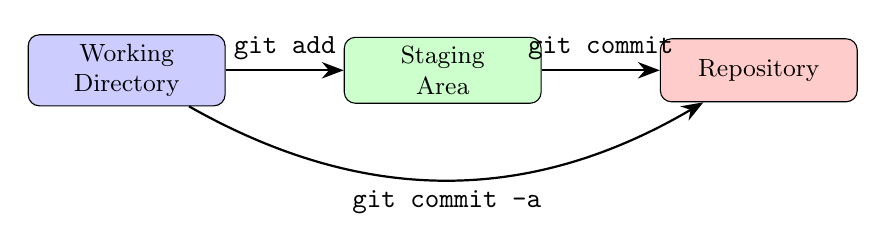
\begin{tikzpicture}[
        stage/.style={draw, rectangle, rounded corners, minimum width=2.5cm, minimum height=0.8cm, align=center, font=\small},
        arrow/.style={-{Stealth[scale=1.2]}, thick, >=stealth}
    ]

    % Stages
    \node[stage, fill=blue!20] (working) {Working\\Directory};
    \node[stage, fill=green!20, right=1.5cm of working] (staging) {Staging\\Area};
    \node[stage, fill=red!20, right=1.5cm of staging] (repo) {Repository};

    % Arrows
    \draw[arrow] (working) -- node[above] {\texttt{git add}} (staging);
    \draw[arrow] (staging) -- node[above] {\texttt{git commit}} (repo);
    \draw[arrow, bend right=30] (working) to node[below] {\texttt{git commit -a}} (repo);

    \end{tikzpicture}
  \end{center}

  \vspace{0.5em}
  \begin{center}
    \begin{minipage}{0.9\textwidth}
    \footnotesize
    \begin{description}
      \item[Working Directory] Your files on disk
      \item[Staging Area] What will be committed
      \item[Repository] Your committed snapshots
    \end{description}
    \end{minipage}
  \end{center}
\end{frame}

% Git Key Features
\begin{frame}{Key Features of Git}
  \begin{columns}
    \begin{column}{0.48\textwidth}
      \begin{block}{Core Capabilities}
        \begin{itemize}
          \item Complete project history
          \item Offline functionality
          \item Branching and merging
          \item Data integrity
        \end{itemize}
      \end{block}
    \end{column}
    \begin{column}{0.48\textwidth}
      \begin{center}
        \includegraphics[width=0.5\textwidth]{figures/gitLogo.png}
      \end{center}
    \end{column}
  \end{columns}
\end{frame}

% Git Advantages
\begin{frame}{Why Choose Git?}
  \begin{columns}
    \begin{column}{0.48\textwidth}
      \begin{block}{Key Advantages}
        \begin{itemize}
          \item Distributed workflow
          \item Fast performance
          \item Strong community support
          \item Cross-platform compatibility
        \end{itemize}
      \end{block}
    \end{column}
    \begin{column}{0.48\textwidth}
      \begin{exampleblock}{Fun Fact}
        The name "Git" is British slang meaning "unpleasant person" - a playful joke by Linus Torvalds!
      \end{exampleblock}
      \vspace{0.5em}
      \begin{alertblock}{Industry Standard}
        Git has become the de facto standard for version control in software development.
      \end{alertblock}
    \end{column}
  \end{columns}
\end{frame}

% Core Git Concepts - Part 1
\begin{frame}{Core Git Concepts: The Basics}
  \begin{columns}
    \begin{column}{0.48\textwidth}
      \begin{block}{Key Components}
        \begin{description}
          \item[Repository] Your project's folder
          \item[Commit] A saved "checkpoint"
          \item[Branch] Parallel version
          \item[Remote] Cloud version (GitHub)
        \end{description}
      \end{block}
      
      \begin{center}
      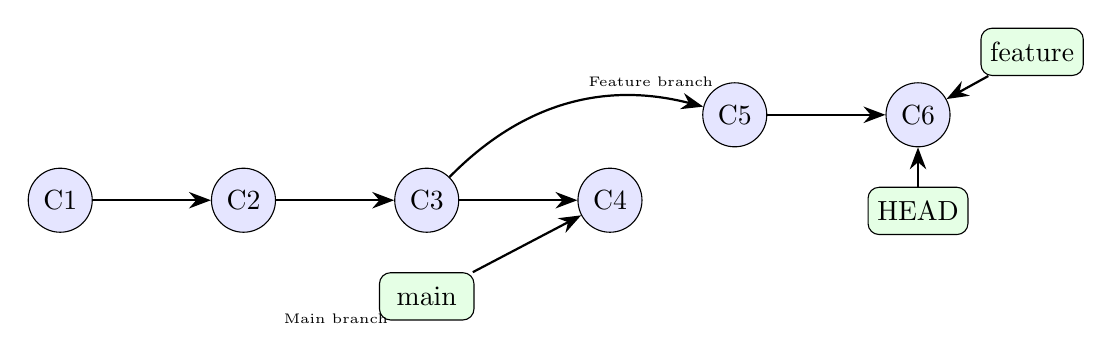
\begin{tikzpicture}[
          commit/.style={circle, draw, fill=blue!10, minimum size=0.7cm},
          branch/.style={rectangle, draw, fill=green!10, rounded corners, minimum width=1.2cm, minimum height=0.6cm},
          arrow/.style={-{Stealth[scale=1.2]}, thick, >=stealth},
          node distance=0.8cm and 1.5cm
      ]
      
      % Commits
      \node[commit] (c1) {C1};
      \node[commit, right=of c1] (c2) {C2};
      \node[commit, right=of c2] (c3) {C3};
      \node[commit, right=of c3] (c4) {C4};
      \node[commit, above right=0.5cm and 1cm of c4] (c5) {C5};
      \node[commit, right=of c5] (c6) {C6};
      
      % Branches
      \node[branch, below=0.5cm of c3] (main) {main};
      \node[branch, above right=0.2cm and 0.5cm of c6] (feature) {feature};
      \node[branch, below=0.5cm of c6] (head) {HEAD};
      
      % Arrows between commits
      \draw[arrow] (c1) -- (c2);
      \draw[arrow] (c2) -- (c3);
      \draw[arrow] (c3) -- (c4);
      \draw[arrow] (c3) to [bend left=30] (c5);
      \draw[arrow] (c5) -- (c6);
      
      % Branch pointers
      \draw[arrow] (main) -- (c4);
      \draw[arrow] (feature) -- (c6);
      \draw[arrow] (head) -- (c6);
      
      % Labels
      \node[text width=3cm, align=center, font=\tiny] at (3.5,-1.5) {Main branch};
      \node[text width=3cm, align=center, font=\tiny] at (7.5,1.5) {Feature branch};
      
      \end{tikzpicture}
      \end{center}
    \end{column}
    
    \begin{column}{0.48\textwidth}
      \begin{exampleblock}{Video Game Analogy}
        \begin{itemize}
          \item Commits = Save points
          \item Branches = Story paths
          \item Remote = Cloud save
        \end{itemize}
      \end{exampleblock}
      
      \vspace{1em}
      
      \begin{center}
        [Space for workflow diagram]
      \end{center}
    \end{column}
  \end{columns}
\end{frame}

% Core Git Concepts - Part 2
\begin{frame}{Git Workflow}
  \begin{block}{Understanding Git Workflow}
    Git's workflow is built around three main areas that help track and manage changes in your project. This structure ensures version control and collaboration efficiency.
  \end{block}

  \vspace{0.5em}
  \begin{block}{The Basic Cycle}
    \begin{enumerate}
      \item Modify files in working directory
      \item Stage changes \texttt{git add}
      \item Commit changes \texttt{git commit}
    \end{enumerate}
  \end{block}
  
  \begin{columns}
    \begin{column}{0.48\textwidth}
      \begin{block}{Working Directory}
        Where you make changes to files
      \end{block}
    \end{column}
    \begin{column}{0.48\textwidth}
      \begin{block}{Staging Area}
        Preview of next commit
      \end{block}
    \end{column}
  \end{columns}
  
  \vspace{1em}
  \begin{center}
    [Space for workflow visualization]
  \end{center}
\end{frame}

% Essential Git Commands - Part 1
\begin{frame}{Essential Git Commands: Getting Started}
  \begin{columns}
    \begin{column}{0.48\textwidth}
      \begin{block}{Repository Setup}
        \begin{description}
          \item[\texttt{git init}] Start new repo
          \item[\texttt{git clone}] Copy existing repo
          \item[\texttt{git status}] Check status
        \end{description}
      \end{block}
      
      \begin{center}
        [Space for init/clone diagram]
      \end{center}
    \end{column}
    
    \begin{column}{0.48\textwidth}
      \begin{exampleblock}{Example}
        \small
        \texttt{\textdollar{} git init}
        
        \texttt{\textdollar{} echo "\# My Project" > README.md}
        
        \texttt{\textdollar{} git add README.md}
        
        \texttt{\textdollar{} git commit -m "Initial commit"}
      \end{exampleblock}
    \end{column}
  \end{columns}
\end{frame}

% Essential Git Commands - Part 2
\begin{frame}{Essential Git Commands: Daily Work}
  \begin{columns}
    \begin{column}{0.48\textwidth}
      \begin{block}{Basic Commands}
        \begin{description}
          \item[\texttt{git add}] Stage changes
          \item[\texttt{git commit}] Save changes
          \item[\texttt{git log}] View history
          \item[\texttt{git diff}] See changes
        \end{description}
      \end{block}
      
      \vspace{1em}
      \begin{center}
        [Space for command examples]
      \end{center}
    \end{column}
    
    \begin{column}{0.48\textwidth}
      \begin{block}{Useful Options}
        \begin{description}
          \item[\texttt{git status -s}] Compact status
          \item[\texttt{git log --oneline}] Compact log
          \item[\texttt{git commit -am}] Add \& commit
        \end{description}
      \end{block}
      
      \vspace{1em}
      \begin{center}
        [Space for more examples]
      \end{center}
    \end{column}
  \end{columns}
\end{frame}

\begin{frame}{Hands-on Exercise}
  \begin{block}{Task: Create Your First Repository}
    \begin{enumerate}
      \item Create a new directory: \texttt{mkdir my-first-repo}
      \item Navigate into it: \texttt{cd my-first-repo}
      \item Initialize Git: \texttt{git init}
      \item Create a README.md file with your project description
      \item Stage the file: \texttt{git add README.md}
      \item Commit your changes: \texttt{git commit -m "Initial commit"}
    \end{enumerate}
  \end{block}
  
  \begin{alertblock}{Check Your Work}
    Run \texttt{git status} to verify your changes are committed
  \end{alertblock}
\end{frame}

\begin{frame}{Key Takeaways}
  \begin{block}{What We've Learned}
    \begin{itemize}
      \item Version control is essential for tracking changes
      \item Git provides a powerful way to manage project history
      \item Basic workflow: modify → stage → commit
    \end{itemize}
  \end{block}
  
  \begin{block}{Next Steps}
    \begin{itemize}
      \item Practice basic Git commands
      \item Explore more Git features
      \item In the next session: Branching and Merging
    \end{itemize}
  \end{block}
\end{frame}

%==================================
\section{Session 2: Advanced Git \& GitHub}

% Session Objectives
\begin{frame}{Session 2: What You'll Learn}
  \begin{columns}
    \begin{column}{0.48\textwidth}
      \begin{block}{Advanced Git}
        \begin{itemize}
          \item Branching and merging
          \item Undoing changes
          \item Using .gitignore
        \end{itemize}
      \end{block}
      
      \begin{center}
        [Space for Git workflow diagram]
      \end{center}
    \end{column}
    
    \begin{column}{0.48\textwidth}
      \begin{block}{GitHub Basics}
        \begin{itemize}
          \item Creating repositories
          \item Pushing code
          \item Basic collaboration
        \end{itemize}
      \end{block}
      
      \begin{center}
        [Space for GitHub screenshot]
      \end{center}
    \end{column}
  \end{columns}
\end{frame}

% What is Branching?
\begin{frame}{What is Branching?}
  \begin{block}{Parallel Universes for Your Code}
    Branching allows you to create separate lines of development that can evolve independently.
    
    \begin{itemize}
      \item \textbf{Isolation}: Work on features/fixes without affecting the main codebase
      \item \textbf{Experimentation}: Try new ideas safely
      \item \textbf{Collaboration}: Multiple people can work simultaneously
      \item \textbf{Organization}: Keep different work streams separate
    \end{itemize}
  \end{block}
  
  \vspace{0.5cm}
  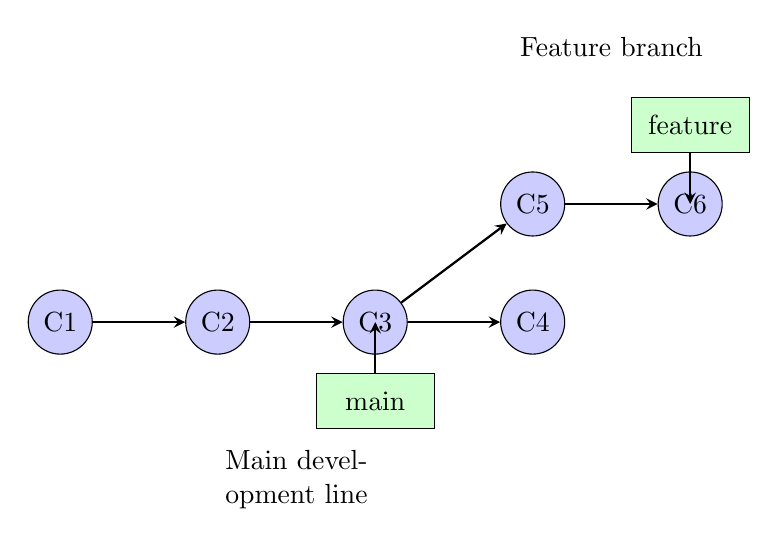
\begin{tikzpicture}[
      commit/.style={circle, draw, fill=blue!20, minimum size=0.7cm},
      branch/.style={rectangle, draw, fill=green!20, minimum width=1.5cm, minimum height=0.7cm},
      arrow/.style={->, >=stealth, thick}
    ]
    % Commits
    \node[commit] (c1) at (0,0) {C1};
    \node[commit] (c2) at (2,0) {C2};
    \node[commit] (c3) at (4,0) {C3};
    \node[commit] (c4) at (6,0) {C4};
    \node[commit] (c5) at (6,1.5) {C5};
    \node[commit] (c6) at (8,1.5) {C6};
    
    % Branches
    \node[branch] (main) at (4,-1) {main};
    \node[branch] (feature) at (8,2.5) {feature};
    
    % Arrows between commits
    \draw[arrow] (c1) -- (c2);
    \draw[arrow] (c2) -- (c3);
    \draw[arrow] (c3) -- (c4);
    \draw[arrow] (c3) -- (c5);
    \draw[arrow] (c5) -- (c6);
    
    % Branch pointers
    \draw[arrow] (main) -- (4,0);
    \draw[arrow] (feature) -- (8,1.5);
    
    % Labels
    \node[text width=3cm, align=center] at (3,-2) {Main development line};
    \node[text width=3cm, align=center] at (7,3.5) {Feature branch};
  \end{tikzpicture}
\end{frame}

% Advanced Git - Part 1
\begin{frame}{Working with Branches}
  \begin{block}{What are Git Branches?}
    Git branches are independent lines of development that allow you to work on different features, fixes, or experiments without affecting the main codebase. They enable parallel development and help organize work efficiently.
  \end{block}

  \vspace{0.5em}
  \begin{columns}
    \begin{column}{0.48\textwidth}
      \begin{block}{Branch Commands}
        \begin{description}
          \item[\texttt{git branch}] List branches
          \item[\texttt{git branch <name>}] Create branch
          \item[\texttt{git checkout <name>}] Switch branch
          \item[\texttt{git merge <name>}] Merge branch
        \end{description}
      \end{block}
    \end{column}
    
    \begin{column}{0.48\textwidth}
      \begin{exampleblock}{Branching Strategy}
        \begin{itemize}
          \item Main/Master - Production code
          \item Develop - Integration branch
          \item Feature/* - New features
          \item Hotfix/* - Quick fixes
        \end{itemize}
      \end{exampleblock}
    \end{column}
  \end{columns}
  
  \vspace{1em}
  \begin{center}
    [Space for branching diagram]
  \end{center}
\end{frame}

% Advanced Git - Part 2
\begin{frame}{Advanced Git: Undoing Changes}
  \begin{block}{What is Undoing Changes?}
    Git provides powerful tools to undo changes at different stages of your workflow. Understanding these tools helps you recover from mistakes and maintain a clean project history.
  \end{block}

  \vspace{0.5em}
  \begin{columns}
    \begin{column}{0.48\textwidth}
      \begin{block}{Undo Commands}
        \begin{description}
          \item[\texttt{git restore <file>}] Discard changes
          \item[\texttt{git revert <commit>}] Create undo commit
          \item[\texttt{git reset}] Move branch pointer
          \item[\texttt{git clean}] Remove untracked files
        \end{description}
      \end{block}
    \end{column}
    
    \begin{column}{0.48\textwidth}
      \begin{alertblock}{Be Careful!}
        Some commands modify history. 
        \begin{itemize}
          \item Use \texttt{revert} for shared branches
          \item Use \texttt{reset} carefully on local branches
        \end{itemize}
      \end{alertblock}
    \end{column}
  \end{columns}
\end{frame}

% GitHub Introduction
\begin{frame}{Introduction to GitHub}
  \begin{columns}
    \begin{column}{0.48\textwidth}
      \begin{block}{What is GitHub?}
        \begin{itemize}
          \item Cloud-based Git hosting
          \item Collaboration platform
          \item Open source community hub
          \item Professional portfolio
        \end{itemize}
      \end{block}
      
      \begin{center}
        [GitHub features]
      \end{center}
    \end{column}
    
    \begin{column}{0.48\textwidth}
      \begin{block}{Key Features}
        \begin{itemize}
          \item Code hosting
          \item Issue tracking
          \item Pull requests
          \item GitHub Actions (CI/CD)
          \item GitHub Pages
        \end{itemize}
      \end{block}
    \end{column}
  \end{columns}
\end{frame}

% Git + GitHub Workflow
\begin{frame}{Git + GitHub Workflow}
  \begin{block}{Basic Commands}
    \begin{description}
      \item[\texttt{git remote add origin <url>}] Connect to GitHub
      \item[\texttt{git push -u origin main}] First push
      \item[\texttt{git clone <url>}] Get existing repo
      \item[\texttt{git pull}] Get latest changes
    \end{description}
  \end{block}
  
  \vspace{1em}
  \begin{center}
    [Workflow diagram: Local $\leftrightarrow$ GitHub]
  \end{center}
  
  \begin{exampleblock}{Best Practice}
    Always \texttt{pull} before you \texttt{push} to avoid conflicts!
  \end{exampleblock}
\end{frame}

% Hands-on Exercise
\begin{frame}{Hands-on: First GitHub Repository}
  \begin{columns}
    \begin{column}{0.48\textwidth}
      \begin{block}{Steps}
        \begin{enumerate}
          \item Create GitHub account
          \item New repository
          \item Connect local repo
          \item Push your code
        \end{enumerate}
      \end{block}
    \end{column}
    
    \begin{column}{0.48\textwidth}
      \begin{center}
        [Screenshot: GitHub new repo]
        
        \vspace{1em}
        [Terminal: git commands]
      \end{center}
    \end{column}
  \end{columns}
  
  \vspace{1em}
  \begin{alertblock}{Remember}
    Don't forget to add a meaningful README.md!
  \end{alertblock}
\end{frame}

%==================================
\section{Session 3: Collaboration on GitHub}

% Session 3 Overview
\begin{frame}{Session 3: Team Collaboration}
  \begin{columns}
    \begin{column}{0.48\textwidth}
      \begin{block}{What We'll Cover}
        \begin{itemize}
          \item Forking repositories
          \item Pull requests
          \item Code reviews
          \item Team workflows
        \end{itemize}
      \end{block}
      
      \begin{center}
        [Collaboration diagram]
      \end{center}
    \end{column}
    
    \begin{column}{0.48\textwidth}
      \begin{block}{Key Benefits}
        \begin{itemize}
          \item Work in parallel
          \item Review changes
          \item Maintain code quality
          \item Document decisions
        \end{itemize}
      \end{block}
      
      \begin{center}
        [Team workflow]
      \end{center}
    \end{column}
  \end{columns}
\end{frame}

% Forking Workflow
\begin{frame}{Forking Workflow}
  \begin{columns}
    \begin{column}{0.48\textwidth}
      \begin{block}{Step 1: Fork}
        \begin{enumerate}
          \item Find a repository on GitHub
          \item Click "Fork" button
          \item Creates your copy
        \end{enumerate}
      \end{block}
      
      \begin{block}{Step 2: Clone}
        \texttt{git clone <your-fork-url>}
      \end{block}
    \end{column}
    
    \begin{column}{0.48\textwidth}
      \begin{center}
        [Fork button screenshot]
        
        \vspace{1em}
        [Repository structure]
      \end{center}
    \end{column}
  \end{columns}
\end{frame}

% Pull Requests
\begin{frame}{Pull Requests}
  \begin{block}{What is a Pull Request?}
    A way to propose and review changes before merging them into the main project.
  \end{block}
  
  \begin{columns}
    \begin{column}{0.48\textwidth}
      \begin{block}{Creating a PR}
        \begin{enumerate}
          \item Push changes to your fork
          \item Click "New Pull Request"
          \item Add description
          \item Request reviews
        \end{enumerate}
      \end{block}
    \end{column}
    
    \begin{column}{0.48\textwidth}
      \begin{center}
        [PR creation flow]
        
        \vspace{1em}
        [Good PR example]
      \end{center}
    \end{column}
  \end{columns}
\end{frame}

% Code Reviews
\begin{frame}{Code Reviews}
  \begin{columns}
    \begin{column}{0.48\textwidth}
      \begin{block}{Reviewing Code}
        \begin{itemize}
          \item Check for bugs and edge cases
          \item Verify code style and best practices
          \item Suggest improvements
          \item Ensure tests are present
        \end{itemize}
      \end{block}
      
      \begin{exampleblock}{Example Review}
        \begin{itemize}
          \item "Consider adding error handling here"
          \item "This could be more efficient if..."
          \item "Don't forget to update the docs"
        \end{itemize}
      \end{exampleblock}
    \end{column}
    
    \begin{column}{0.48\textwidth}
      \begin{block}{Best Practices}
        \begin{itemize}
          \item Be constructive and kind
          \item Explain the 'why' behind suggestions
          \item Keep reviews focused and actionable
          \item Review in a timely manner
        \end{itemize}
      \end{block}
      
      \begin{center}
        [Code review interface]
      \end{center}
    \end{column}
  \end{columns}
\end{frame}

% GitHub Features
\begin{frame}{GitHub Features for Teams}
  \begin{columns}
    \begin{column}{0.45\textwidth}
      \begin{block}{Project Management}
        \begin{description}
          \item[Issues] Track bugs and features
          \item[Projects] Kanban-style boards
          \item[Discussions] Team conversations
          \item[Wiki] Project documentation
        \end{description}
      \end{block}
      
      \begin{block}{Automation}
        \begin{itemize}
          \item GitHub Actions (CI/CD)
          \item Branch protection rules
          \item Auto-merge PRs
          \item Code scanning
        \end{itemize}
      \end{block}
    \end{column}
    
    \begin{column}{0.5\textwidth}
      \begin{center}
        [GitHub features overview]
        
        \vspace{1em}
        \begin{exampleblock}{Team Workflow}
          \begin{enumerate}
            \item Create issue
            \item Branch off main
            \item Make changes
            \item Open PR
            \item Review and discuss
            \item Merge and deploy
          \end{enumerate}
        \end{exampleblock}
        
        \vspace{1em}
        [Workflow visualization]
      \end{center}
    \end{column}
  \end{columns}
\end{frame}

% GitHub Features Table
\begin{frame}{GitHub Features Overview}
  \begin{center}
    \begin{tabular}{ll}
      \textbf{Feature} & \textbf{Description} \\ \hline
      Issues & Track bugs and features \\
      Pull Requests & Suggest and review code changes \\
      Actions & Automate tasks (CI/CD) \\
      Wiki & Project documentation \\
      Projects & Kanban-style task management \\
      Discussions & Team conversations \\
      Security & Vulnerability alerts and Dependabot
    \end{tabular}
  \end{center}
\end{frame}

\begin{frame}{Open Source and Team Projects}
  \begin{columns}
    \begin{column}{0.48\textwidth}
      \begin{block}{Benefits}
        \begin{itemize}
          \item Build a public portfolio
          \item Learn from other developers
          \item Contribute to tools you use
          \item Improve coding skills
        \end{itemize}
      \end{block}
    \end{column}
    
    \begin{column}{0.48\textwidth}
      \begin{block}{Best Practices}
        \begin{itemize}
          
          \item Use branches and PRs to avoid conflicts
          \item Communicate through Issues and Discussions
          \item Follow the project's contribution guidelines
          \item Keep changes focused and well-documented
        \end{itemize}
      \end{block}
    \end{column}
  \end{columns}
\end{frame}

\begin{frame}{Practice Idea}
\begin{itemize}
  \item Work in pairs
  \item One creates a repository, the other forks it
  \item Collaborate using pull requests and issues
\end{itemize}
\end{frame}

%==================================
\section{Conclusion}

\begin{frame}{Conclusion}
\begin{itemize}
  \item You learned what version control is
  \item You mastered Git basics and advanced commands
  \item You discovered GitHub collaboration tools
\end{itemize}

\bigskip
\textbf{Next Steps:}
\begin{itemize}
  \item Practice Git commands every day
  \item Build your portfolio on GitHub
  \item Contribute to open-source projects
\end{itemize}
\end{frame}

\begin{frame}
  \centering
  \Huge{\textbf{Thank You!}}\\[1em]
  \large{Questions or feedback?}
\end{frame}

\end{document}
